\documentclass[apa]{article}
\usepackage[a4paper,top=3cm,bottom=2cm,left=3cm,right=3cm]{geometry}
\usepackage[utf8]{inputenc}
\usepackage{rotating}
\usepackage{amssymb}
\newcommand{\HRule}[1]{\rule{\linewidth}{#1}}


\title{WheniIs under weighting of outcomes while sampling optimal?}
\author{Simon Ciranka, Bernhard Spitzer}
\date{March, 2018}

\begin{document}
\maketitle

\section{Intro}
In economic decision making paradigms participants are asked to decide between two differently valued options that have probabilistic outcomes. Usually this is studied by observing choices between some monetary gambles. This line of research gave rise to some understanding of how people make decisions in general and what kinds of biases may play a role in human decision making. 
Two major findings dominate the research of judgment and decision making in economic choice. First, when people make choices between monetary gambles, they do not represent option values as they are "objectively out there in the world" rather they base their choices on option utilities. The utilities result from compressing or anti-compressing economic values by the means of a power function and may represent lots of things from personality attributes to socioeconomic status. Second, people also seem to represent probabilities not as they re described to them but weight low probabilities more and high probabilities less then an optimal decision maker would do. These and other findings have sparked research programs devoted to investigate the biases that found in human (and rodent) decision making, emphasizing that deviations from normative decision values may be maladaptive. 

It is however also widely accepted that in environments that carry some degree of unpredictability or uncertainty, these biases may prove to be useful heuristics in order to guide the reasonably good choices with low computational effort. Uncertainty can impact any part of human information processing from knowing where i stand in this world, what actions to take in order to pursue goals or what goals i have in the first place \cite{Bach2012}. These sorts of unknowns fall into the domain of epistemic uncertainty. And these unknowns can be tackled via learning. If all uncertainties are resolved they reduce down to risk, describing the general degree of unpredictability of an environment or "outcome uncertainty". In information processing systems the degree of unpredictability has termed noise or entropy and was traditionally treated as problematic.

More recently however the functional role of noisy encoding of states has been discussed in the neuroscientific literature. Noise is an inherent property of the nervous system, and in many domains it has been shown that, other than previously thought, high noise, or uncertainty can lead to  performance increase under certain conditions in perceptual decision making. 
In the following we investigate if the same is true for economic choice and evaluate how learning and decision making "biases" may lead to more stable and normatively "good" choices in some environments. 

\section{Models \& Simulation}
We simulate an experiment in which agents need to infer the outcome probabilities of a gamble and then make a decision between this gamble and a safe
option, that has a higher expected value than the probabilistic option in one half and a lower expected value in the other half of the cases. The
probabilities of the gamble are presented to the agents analogously to drawing marbles from an urn. Here we randomly generated 500 probability values that
informed a binomial distribution. Each trial, the agents perform 500 trials in which it "sees" the outcome of a binomial distribution with $$ N = x*5 \mid
 x \in \mathbb{N} $$. We manipulate the uncertainty of the agent about the actual outcome distribution by varying the amount of evidence the agent is
presented with from 1 to 9. The agent updates its initially uninformative beliefs about the outcome distribution by updating a beta distributions that
represents the possible underlying probabilistic structure of the experiment and the agents uncertainty about it.

 \begin{equation}
 p_i \sim Beta(\alpha + k_i^{\omega} , \beta + (N_i-k_i)^\omega)
 \end{equation}
 
Where $\alpha$ and $\beta$ are set to one, reflecting an uninformative prior. beeing informed about the outcome distribution the agent decides 
The following equation is commonly used as a utility function of a decider.

\begin{equation}
EU_{solo} = p_i*(V_i)^\rho
\end{equation}

Where \(p_i\) now denotes the agents belief about the probability of a success in gamble \(i\) and \(V_i\) it's value in an arbitrary currency. $\rho$ determines the convexity or compression of the utility function with 1 being a linear or risk neutral mapping from expected value to expected utility. Vaules higher than 1 reflect risk seeking policies and values lower than 1 result in risk averse policies in the gain domain. 
The expected Utility of both the safe and the risky option are now passed to a sigmoid function in order to calculate the probability of each individual to choose the risky option.

\begin{equation}
p_{ChooseRisk_{Solo}}=\frac{1}{1+e^-{(EU_{Risk}-EU_{Safe})*\tau}}
\end{equation}

\section{Comments}
The choices of the agent are then compared the the normative right choice via mean squared error. We can see that in many cases for risk averse and risk neutral individuals, a conservative learning bias may actually be beneficial given some degree of decision or late noise.
Of course this project is only at the beginning and we need to think about better choice scenarios. 
As i set up the environment currently, and compute the mean squared error, random choosing would naturally be evaluated well. So we have a special environment and a special case of evaluating performance. Therefore the figures down there look a little bit too good to be true.

\begin{sidewaysfigure}[!ht]
\centering
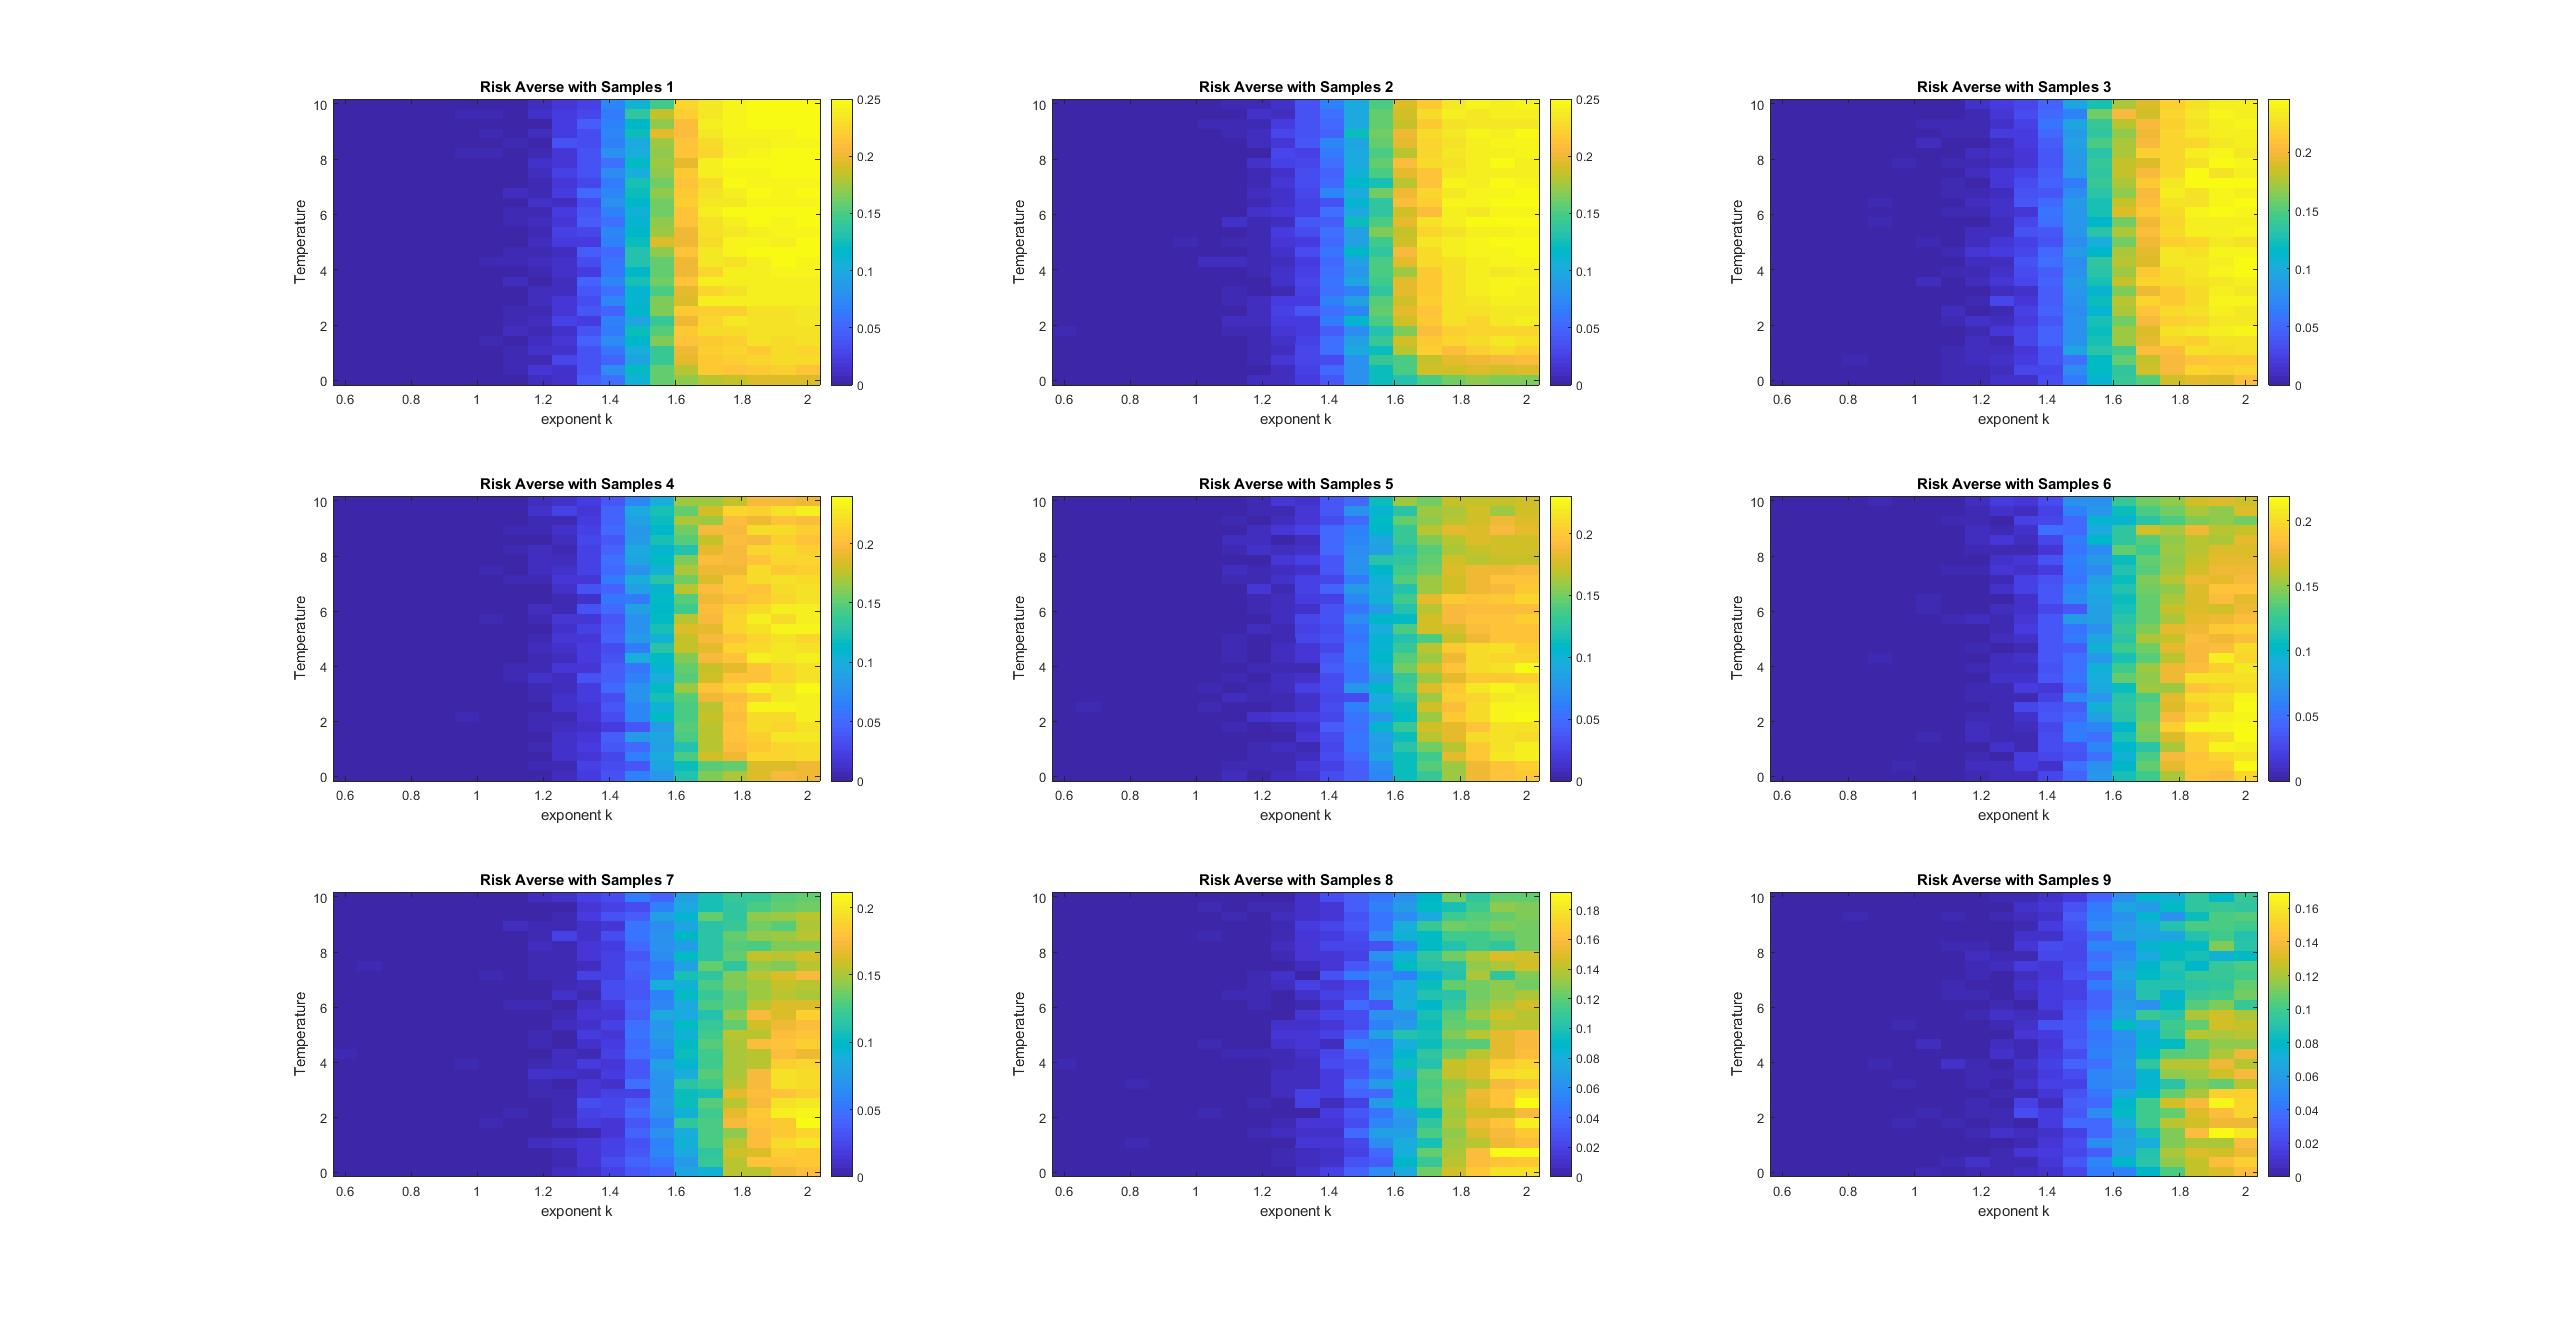
\includegraphics[width=\textwidth]{Risk_Averse.jpg}
\caption{Risk Averse ($\rho = 0.4$) Agent Simulation. The heat is squared error of the mean of the binary choice. Higher temperature refers to an higher $\tau$ parameter, meaning less decision noise. Exp refers to either under or over weighting of the evidence as presented to the agent. Less samples means more uncertainty}
\label{fig:universe}
\end{sidewaysfigure}

\begin{sidewaysfigure}[!ht]
\centering
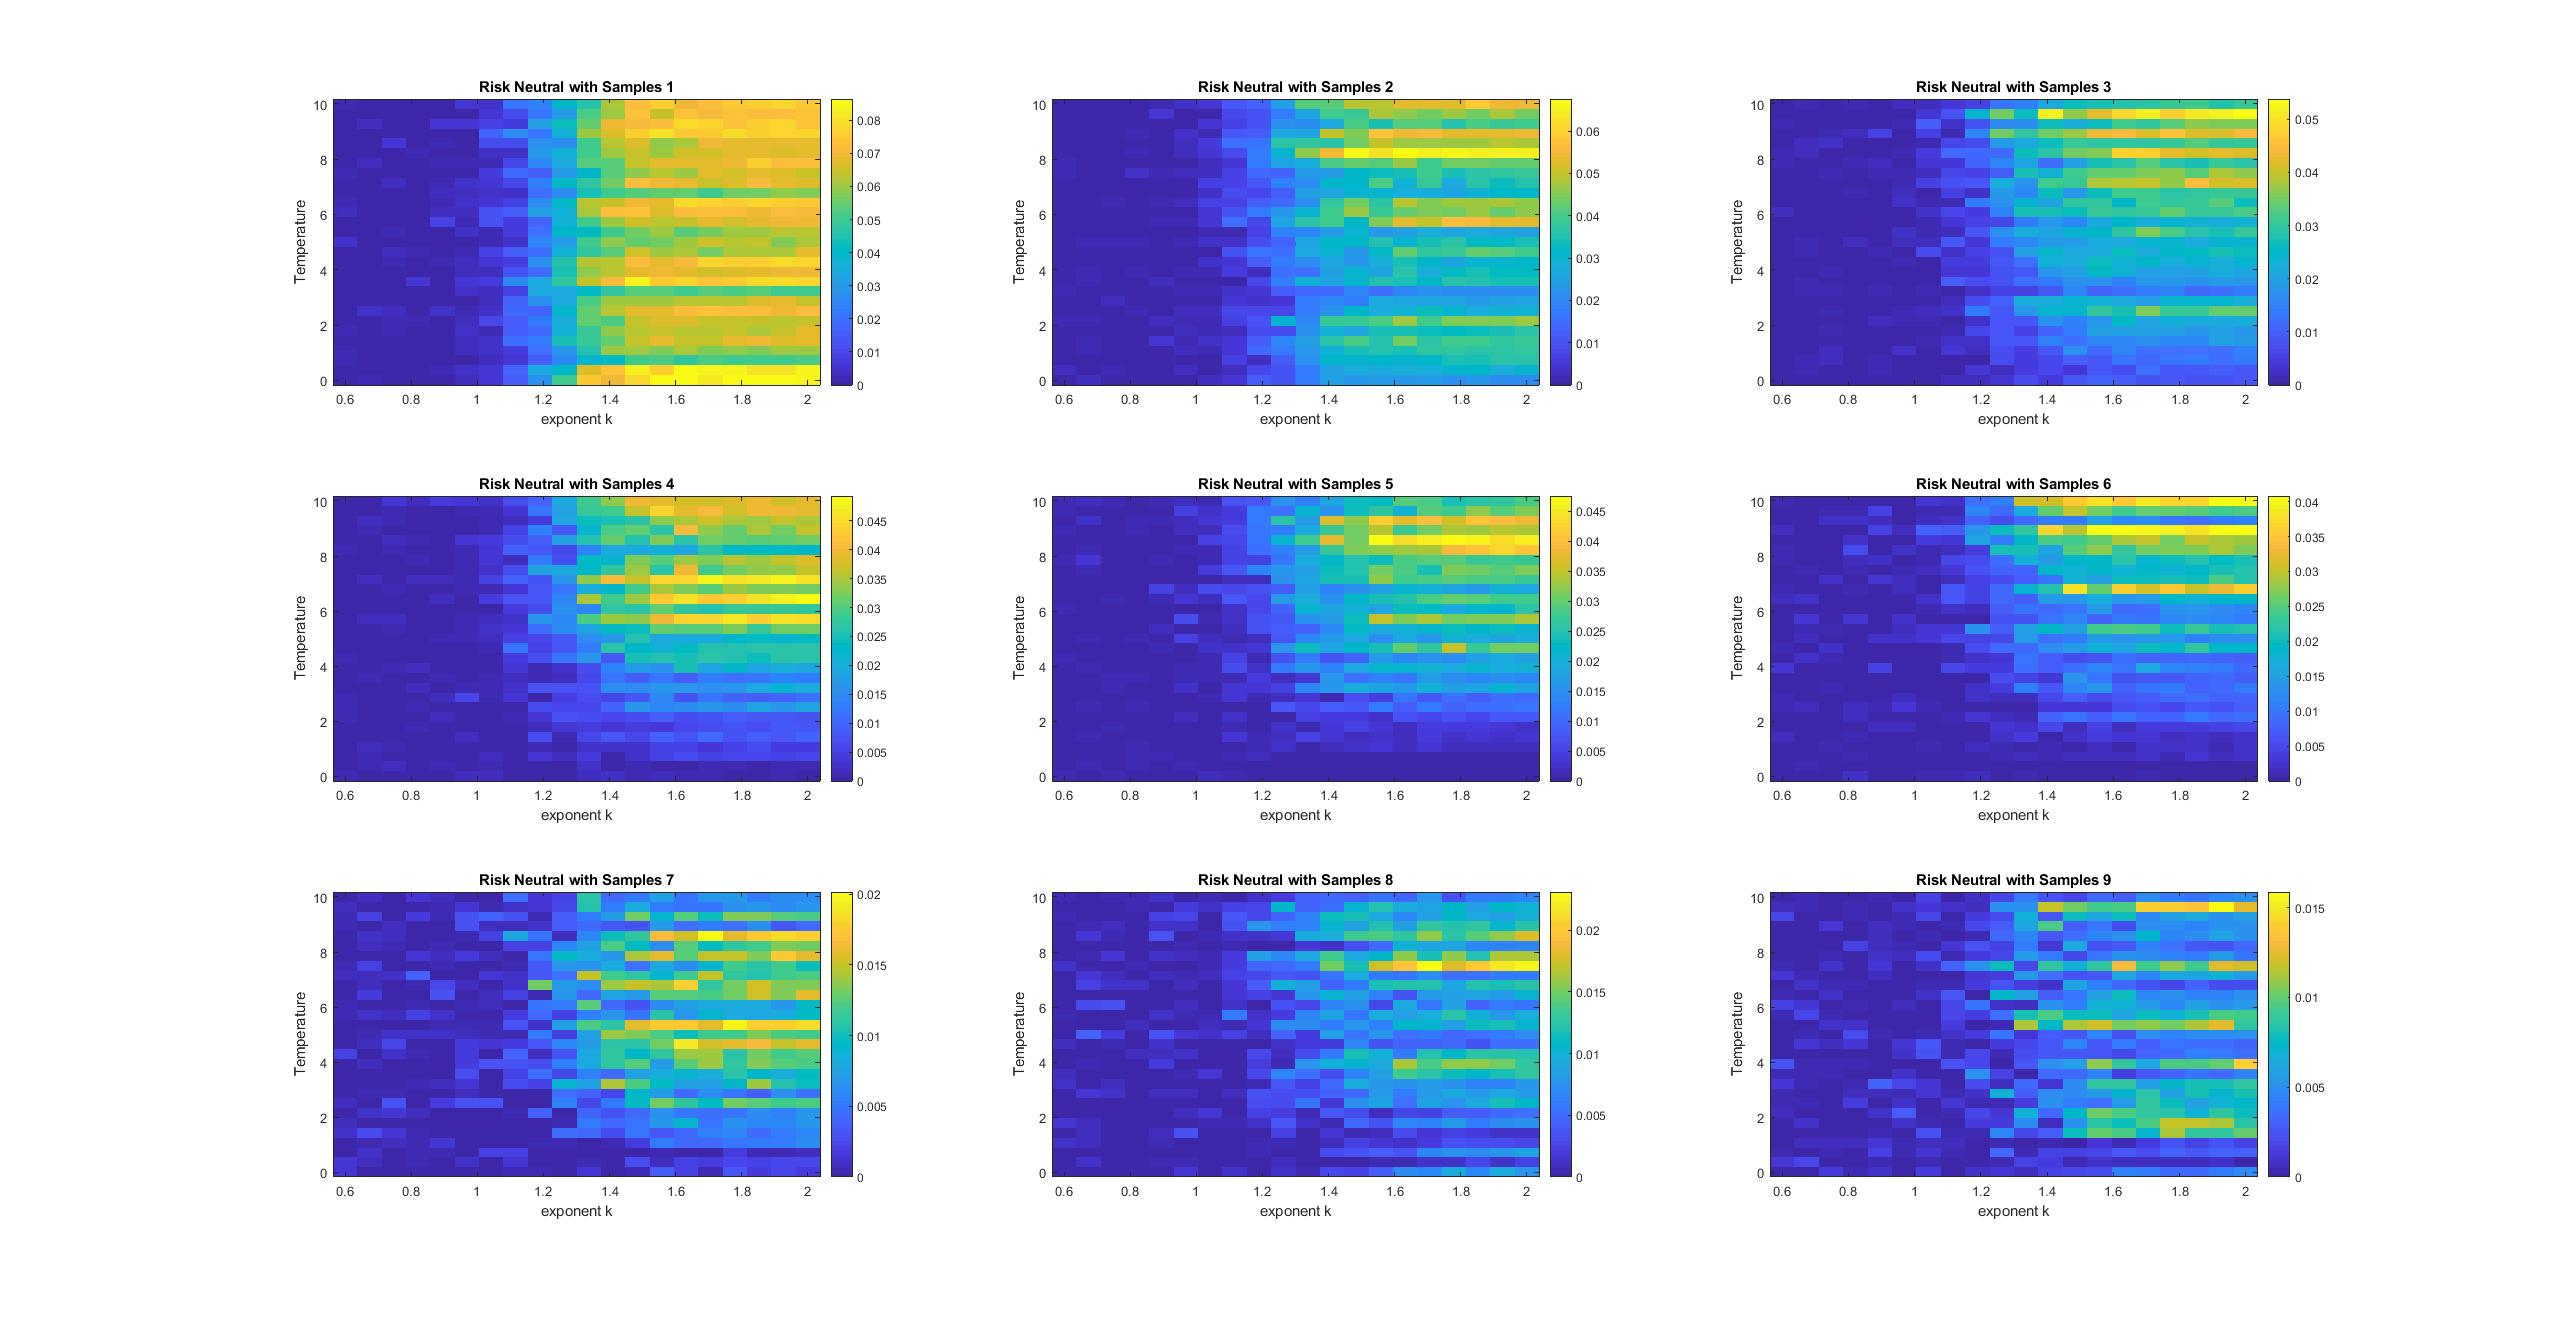
\includegraphics[width=\textwidth]{RiskNeutral.jpg}
\caption{Risk Neutral ($\rho = 1$) Agent Simulation.}
\label{fig:universe}
\end{sidewaysfigure}


\begin{sidewaysfigure}[!ht]
\centering
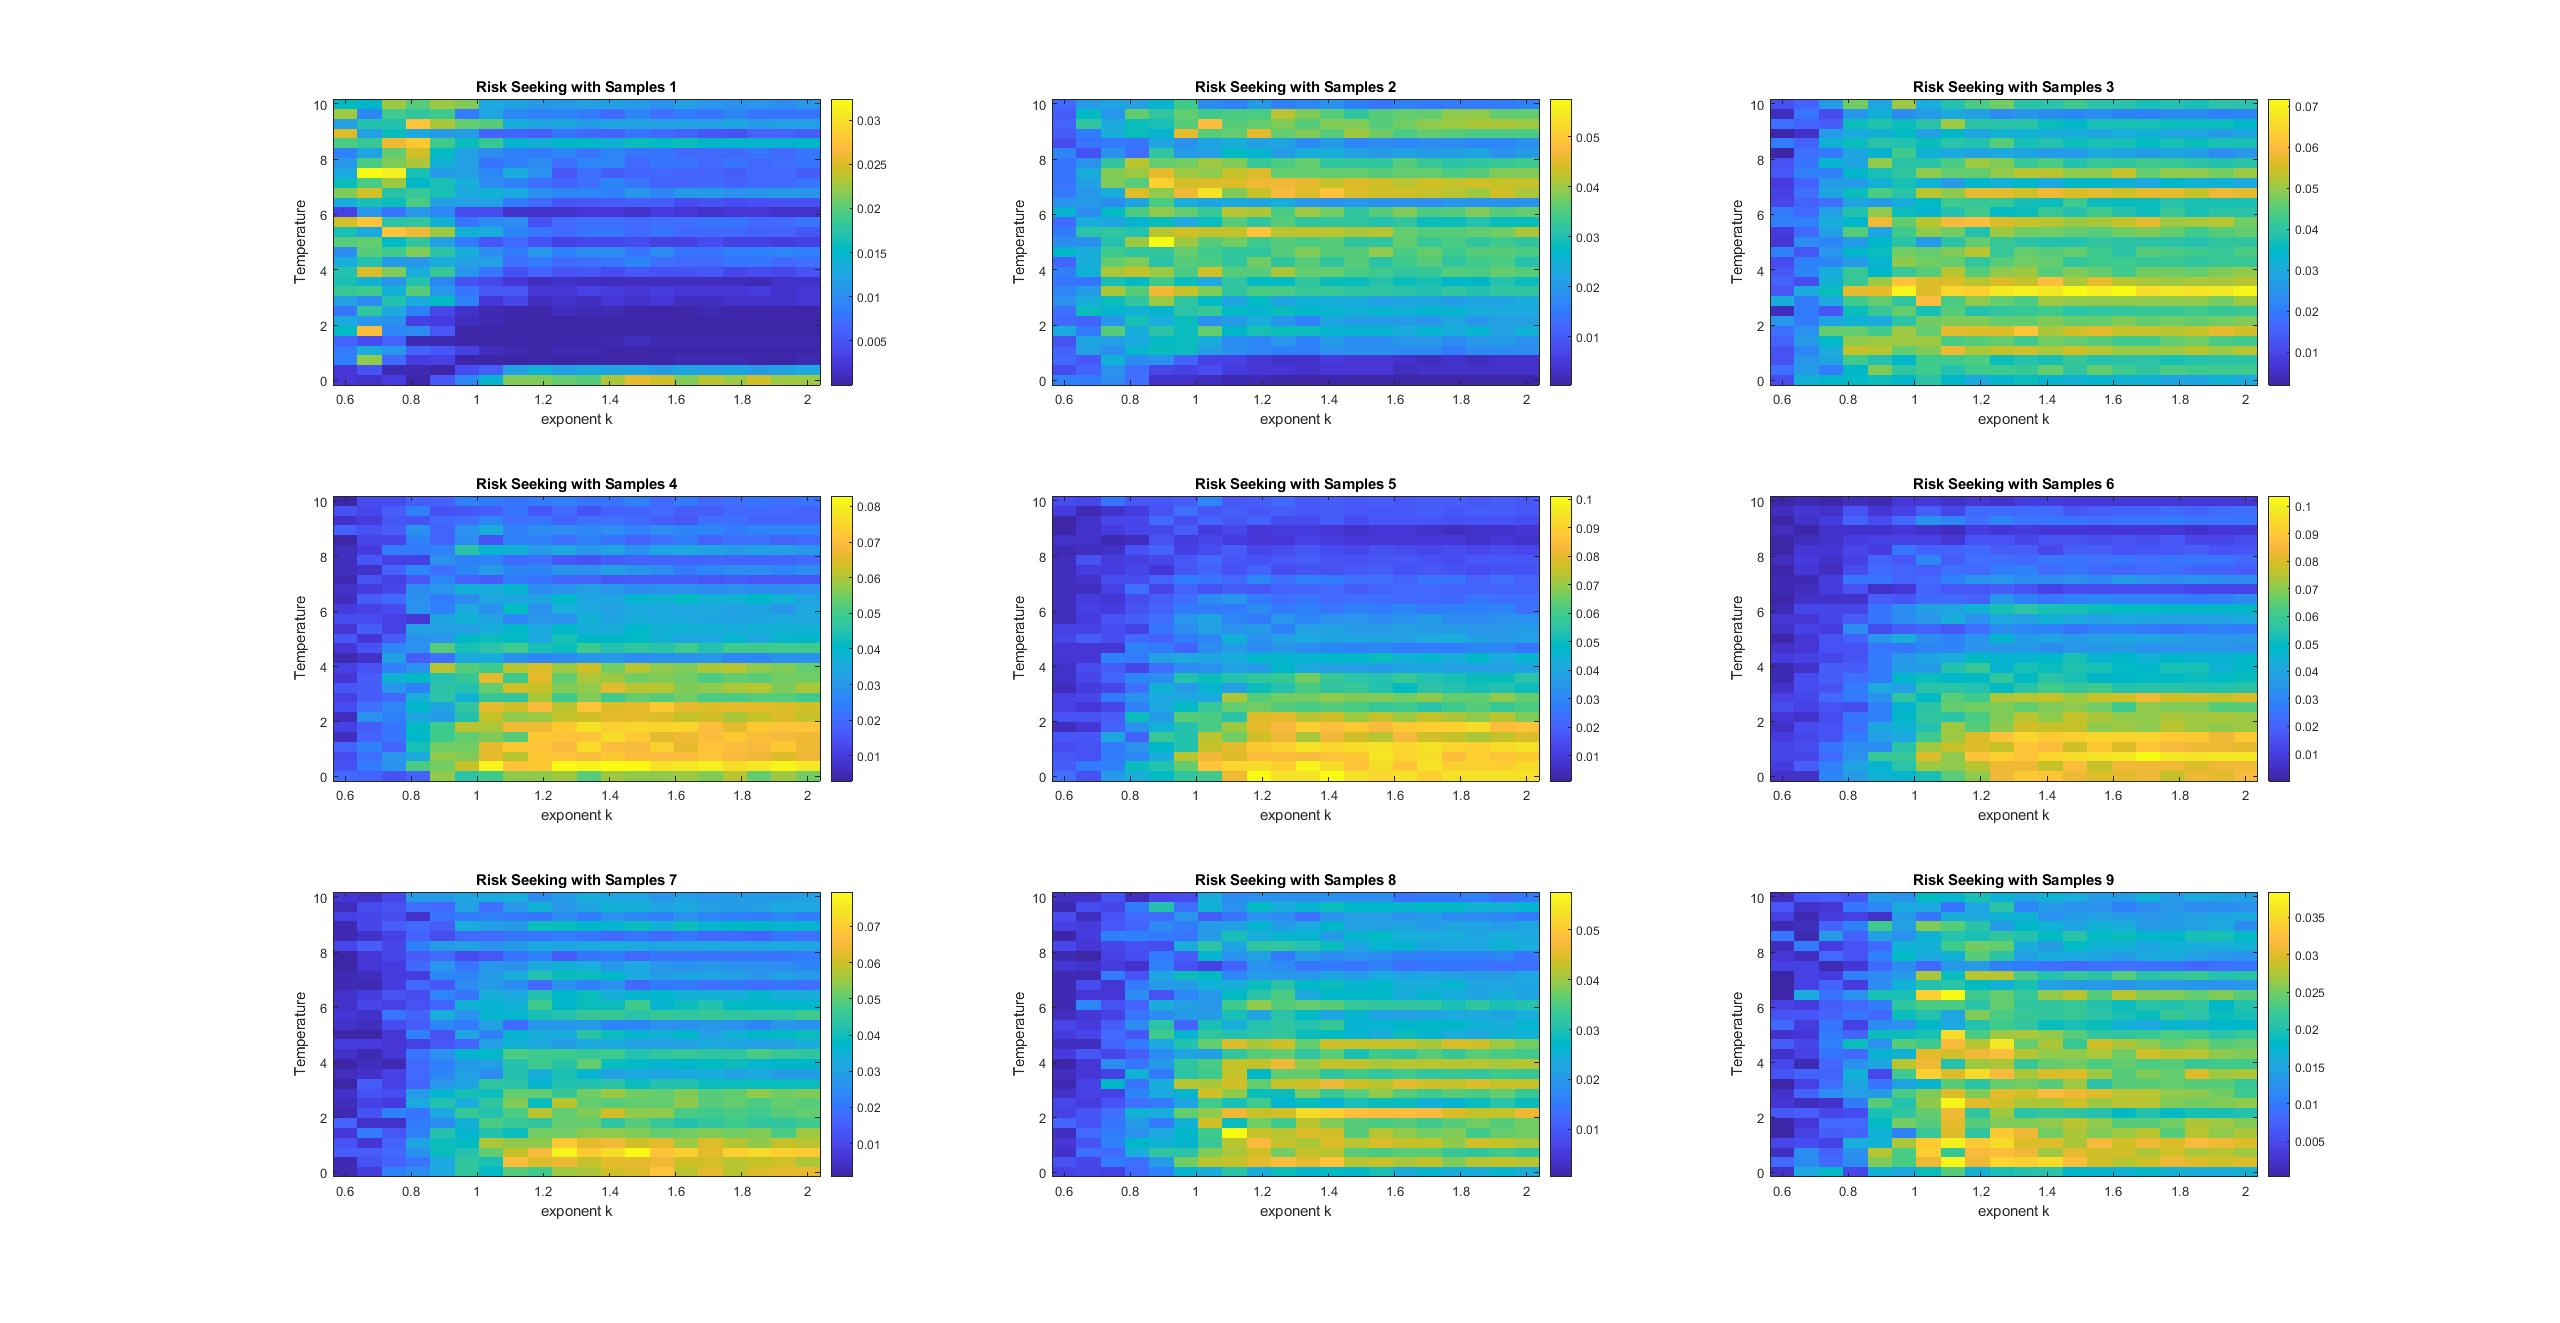
\includegraphics[width=\textwidth]{RiskSeeking.jpg}
\caption{Risk Seeking ($\rho = 1.6$) Agent Simulation.}
\label{fig:universe}
\end{sidewaysfigure}


\section{Conclusion}

\bibliographystyle{plain}
\bibliography{references.bib}
\end{document}
